<<<<<<< HEAD
rs
gdrs
gtfhft
ghstfhdtrhjstr
ht
t
h


=======
\documentclass[]{beamer}
\usepackage[utf8]{inputenc}
\usetheme{Copenhagen}
\usecolortheme{seahorse}

\title{Implementacija osnovnih git komandi}
\author{Adrian Bralic Toth \and Anton Frlan}
\institute{Tehnički Fakultet Rijeka}
\date{2018}

\begin{document}

\frame{\titlepage}

\begin{frame}{git init}

\begin{itemize}
	\setlength\itemsep{2em}
	\item git init stvori .git datoteku te ostale u njoj napravi jos neke datoteke potrebne za rad git-a
	\begin{figure}
\centering
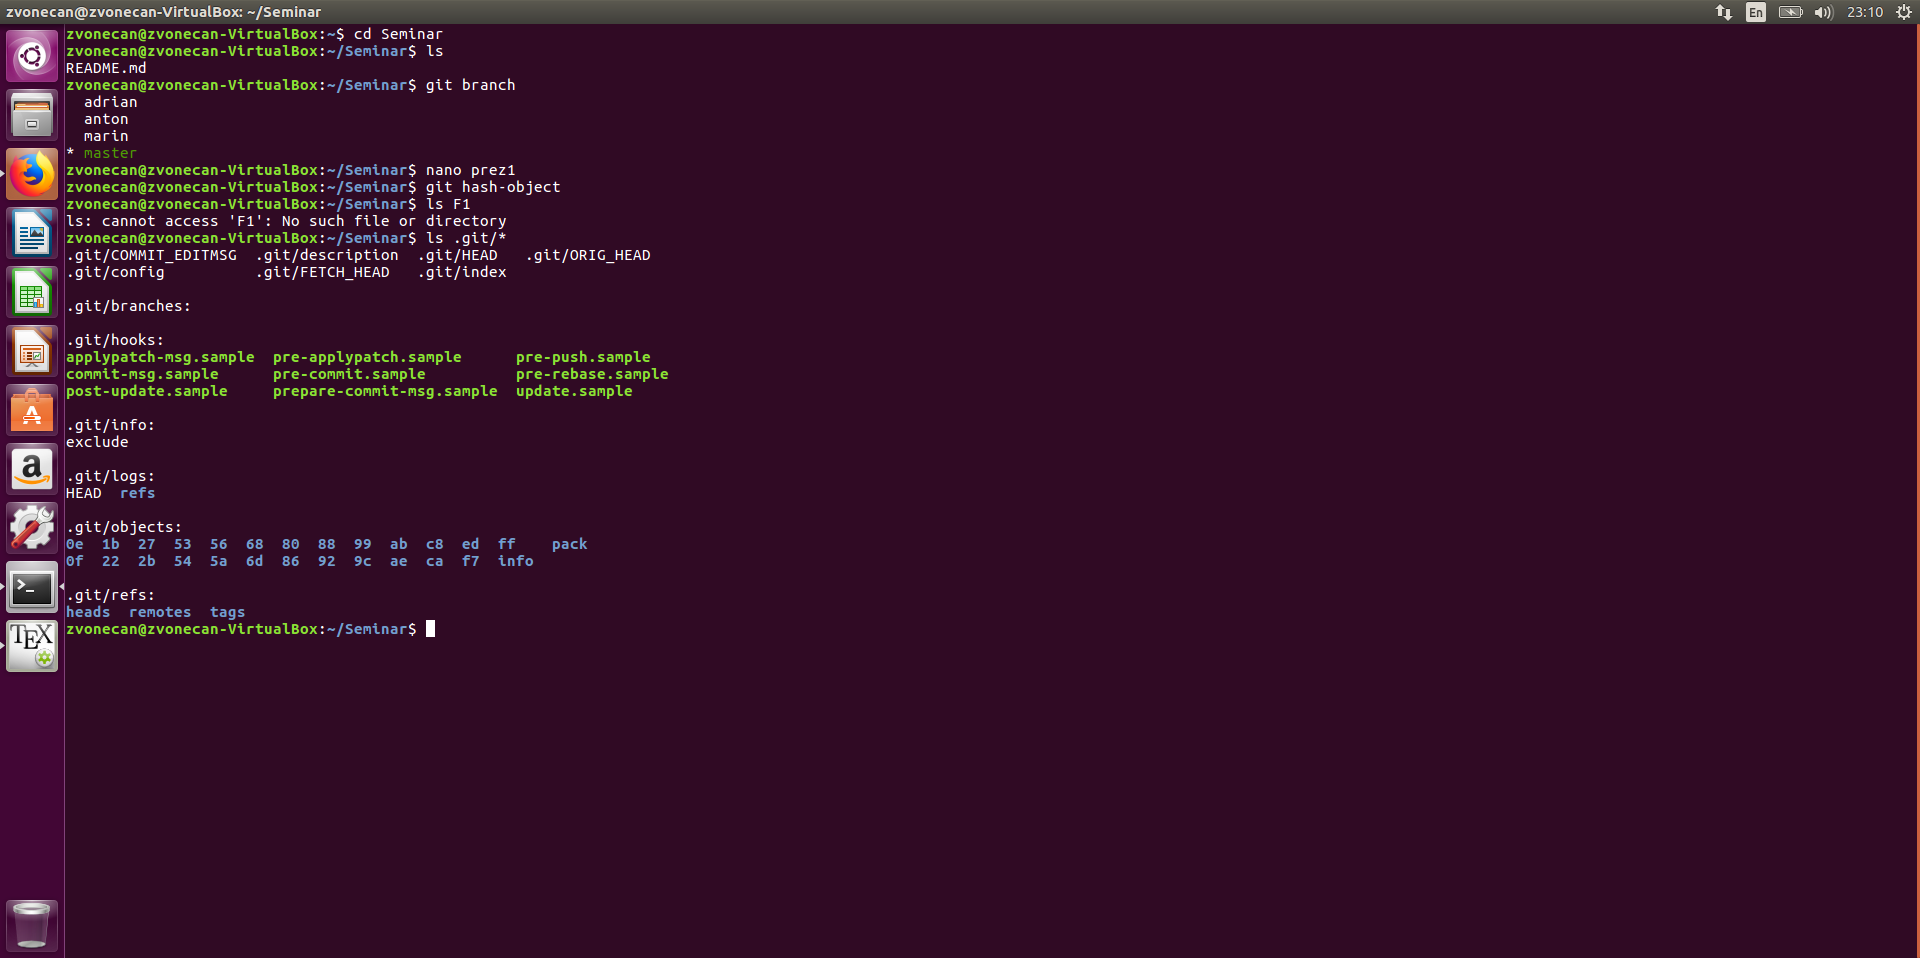
\includegraphics[width=0.9\textwidth]{./slike/git_datoteka.jpg}
\end{figure}
\end{itemize}

\end{frame}


\begin{frame}{git commit}

\begin{itemize}
	\setlength\itemsep{2.5em}
	\item git commit git izvrsava tako da datoteku spremi pod kljuc zvan SHA-1
	\item SHA-1 je kombinacija od 40 malih slova ili brojeva koja sluzi kao pointer na spremljenu datoteku
	\item pomocu komande git hash-object mozemo spremi neki file u git te dodavanjem -w nam git vraca SHA-2 od tog file-a
	\item pomocu git hash-object spremamo neki file pod SHA-2 kao blob i mozemo mu pristupiti samo pomocu SHA-2 kljuca
\end{itemize}

\end{frame}

\begin{frame}{git commit}
\begin{figure}
\centering
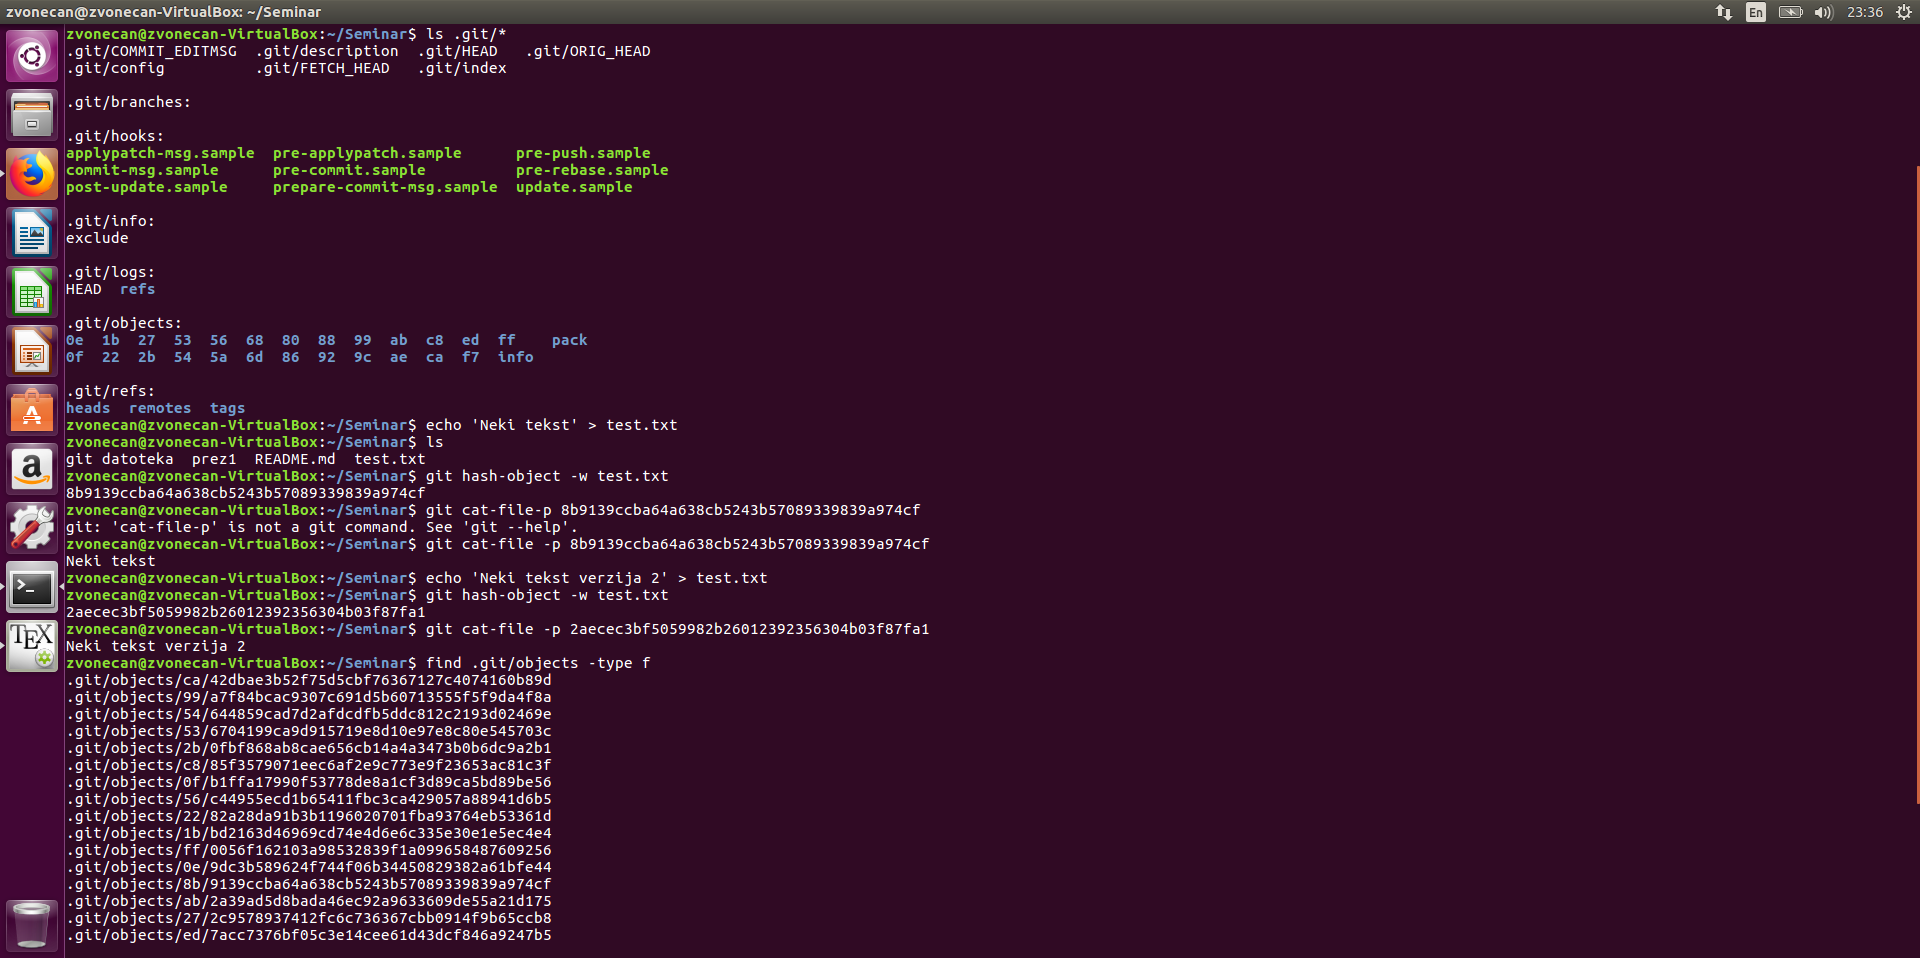
\includegraphics[width=1\textwidth]{./slike/druga_slika.jpg}
\end{figure}

\end{frame}

\begin{frame}{git commit}

\begin{itemize}
	\item git rjesava taj problem pomocu stabala
	\item blob je neki podatak / tekst dok je stablo vise bloboa i barem 2 stablo od kojih 2 stablo ima SHA-2 te datoteke ili stabla koji ga ima
	\begin{figure}
		\centering
	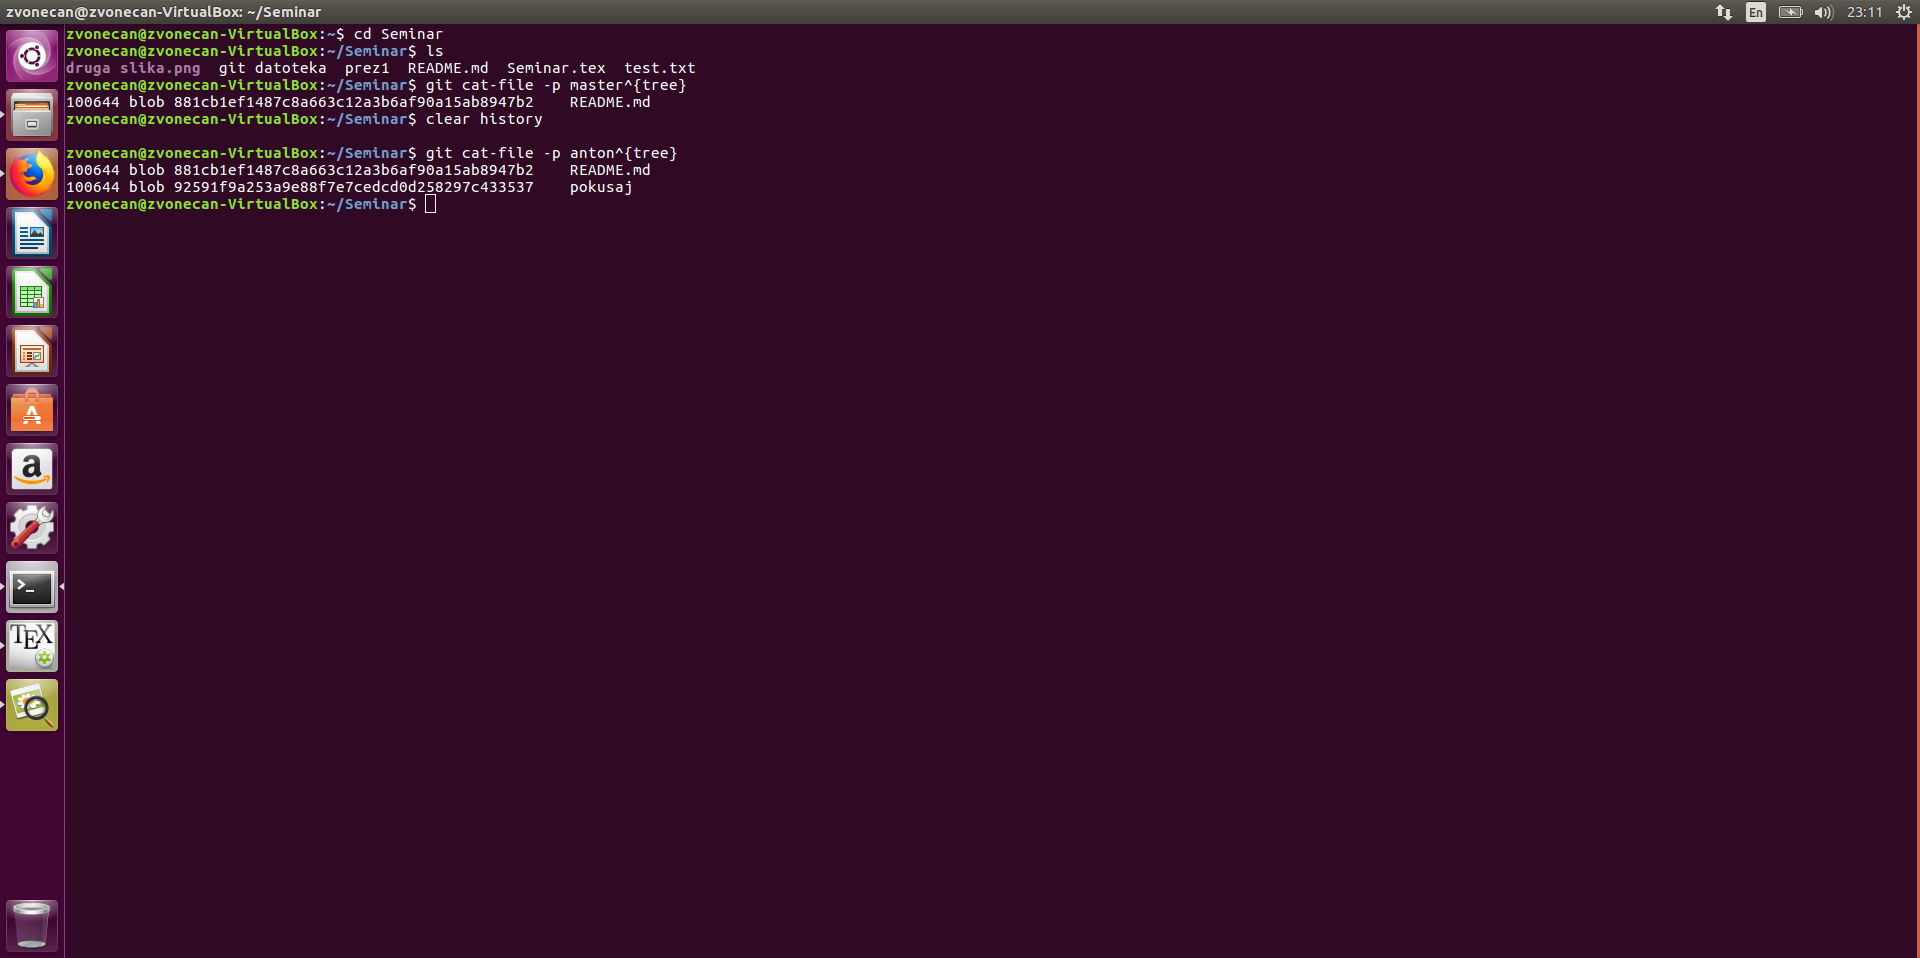
\includegraphics[width=0.8\textwidth]{./slike/treca_slika.jpg}
	\end{figure}
	\item kada git commita file on obicno uzme sto je na stage-u i spremi u jedno stablo ili kombinaciju stabla koji su svi spremljeni pod jedno stablo
\end{itemize}
\end{frame}

\begin{frame}{git stage}

\begin{itemize}
	\item file u gitu stage-amo tako da ga dodamo u pod datoteku index unutar .git datoteke
	\item file dodajemo u index pomocu git update-index --add
	\begin{figure}
		\centering
	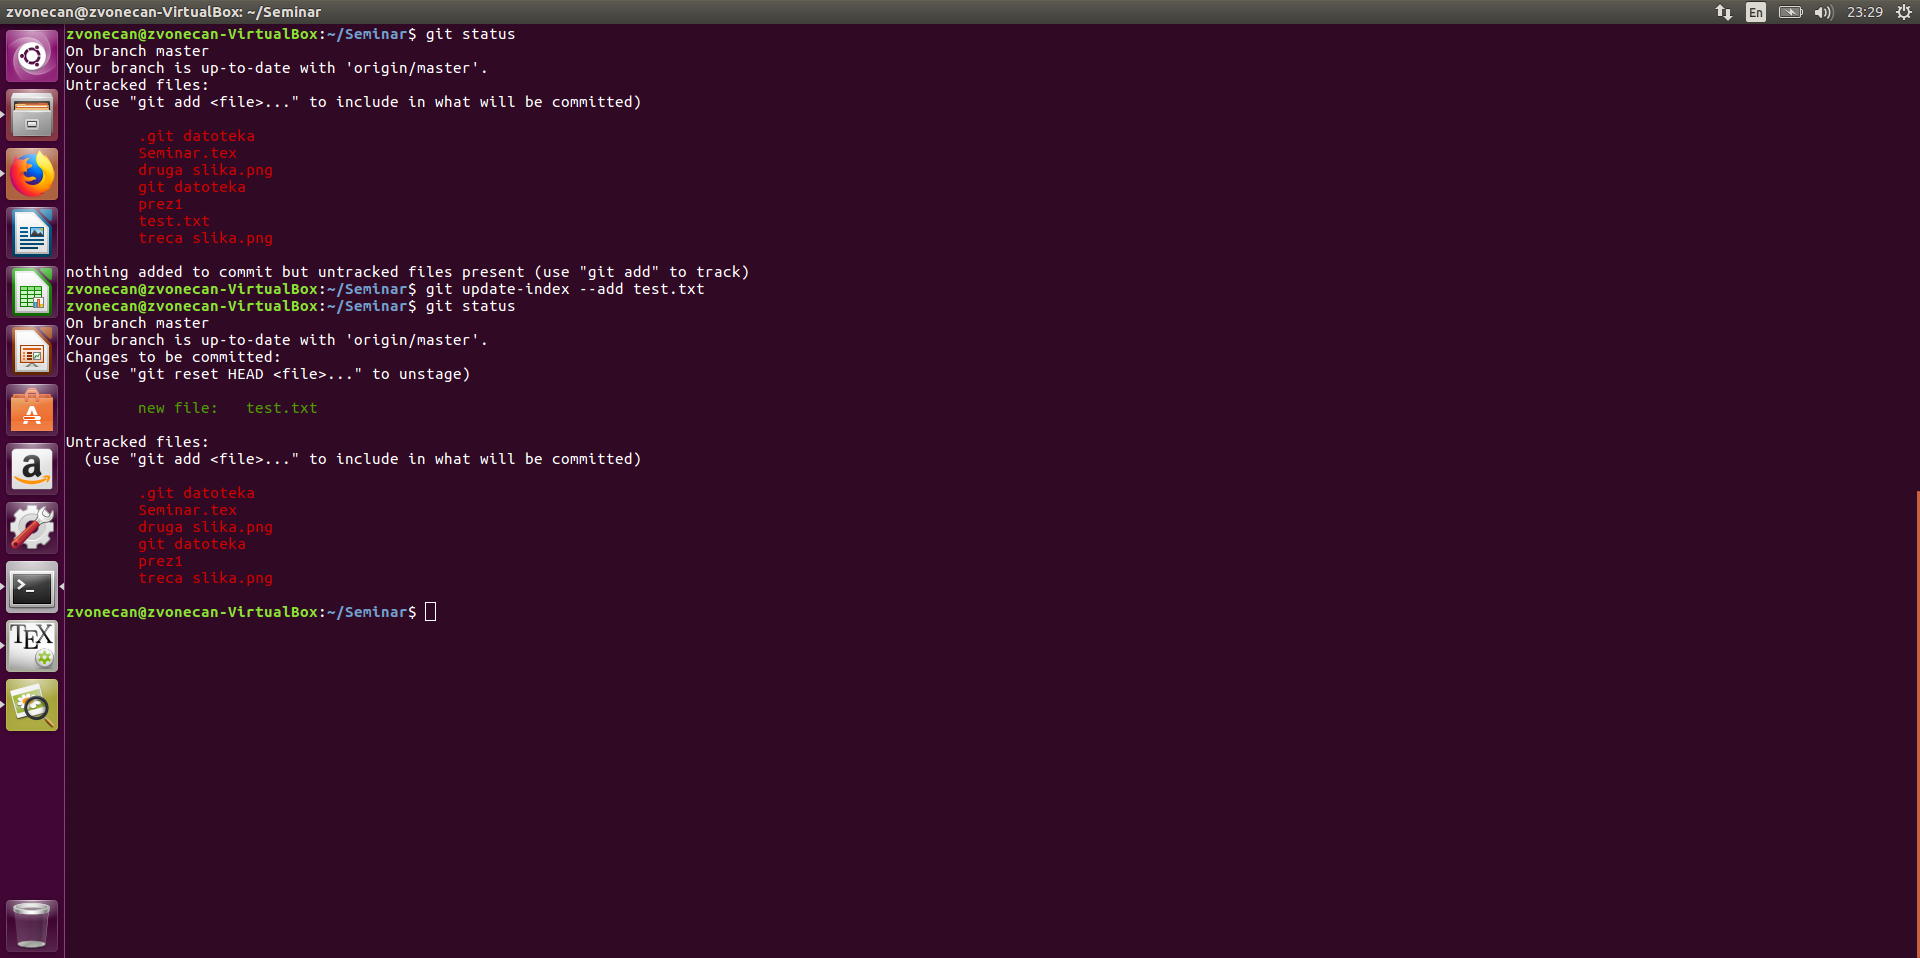
\includegraphics[width=0.8\textwidth]{./slike/cetvrta_slika.jpg}
	\end{figure}
	\item ako zelimo stage-a neki prijasnji commit prije imena file-a moramo doda --cached i SHA-2 tog file-a
	\item sad mozemo napraviti istu stvar sto git radi sa file-ovima u indexu , stablo
	\begin{figure}
		\centering
	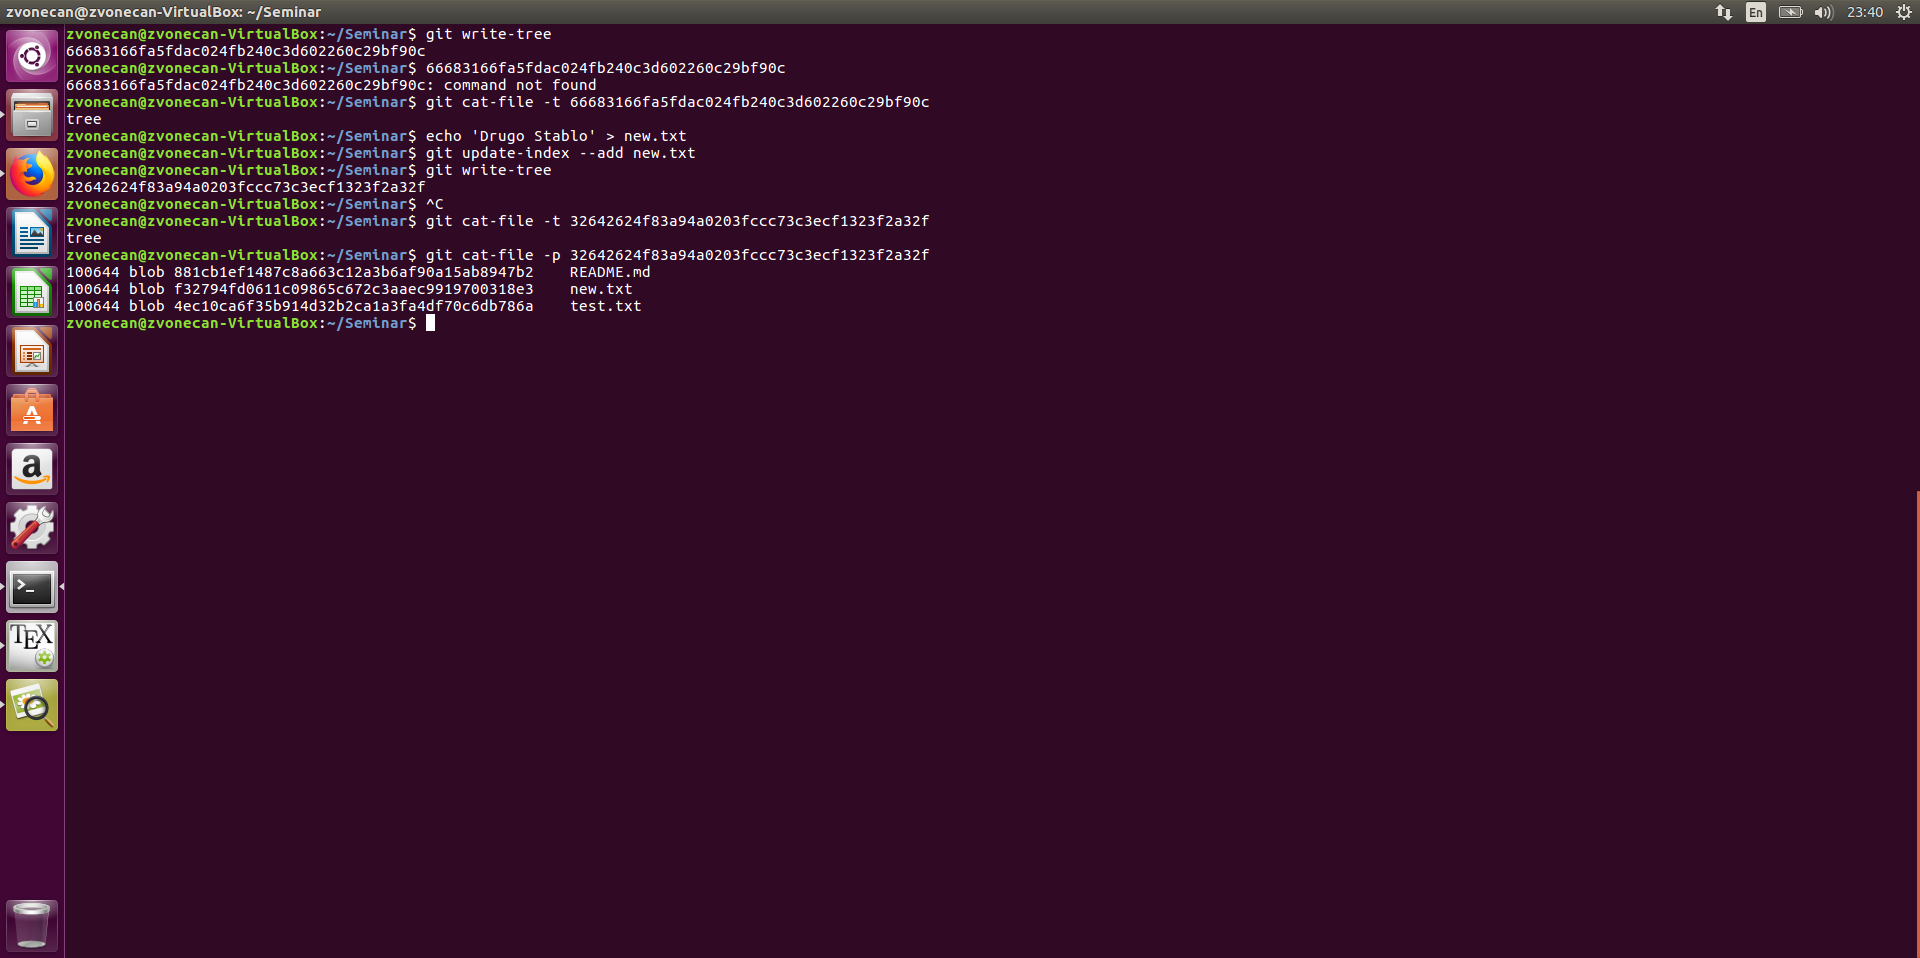
\includegraphics[width=1\textwidth]{./slike/peta_slika.jpg}
	\end{figure}
		
\end{itemize}


\end{frame}

\begin{frame}{git stage}
	\begin{figure}
		\centering
	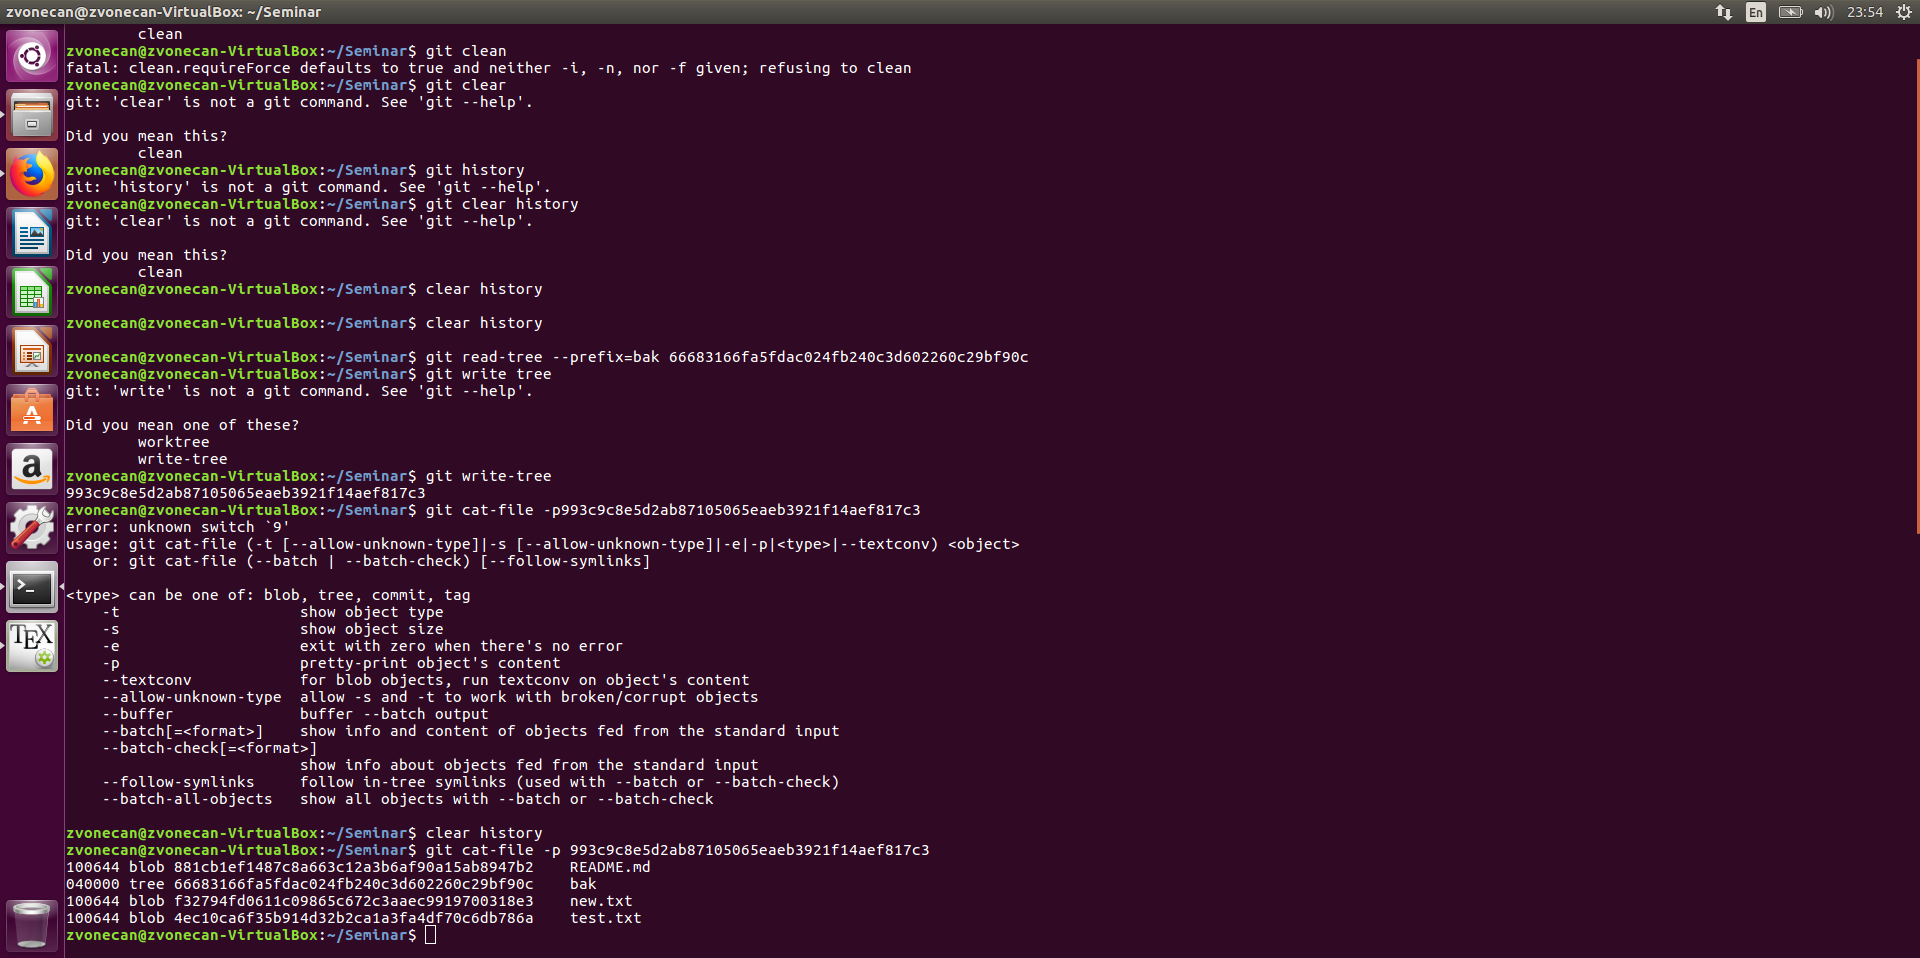
\includegraphics[width=1\textwidth]{./slike/sesta_slika.jpg}
	\end{figure}


\end{frame}

\begin{frame}{git commit}

\begin{itemize}
	\item sad samo commitamo stablo koje smo napravili te smo izvrsili istu stvar koju git napravi kada nesto add-amo i commit-amo
	\begin{figure}
		\centering
	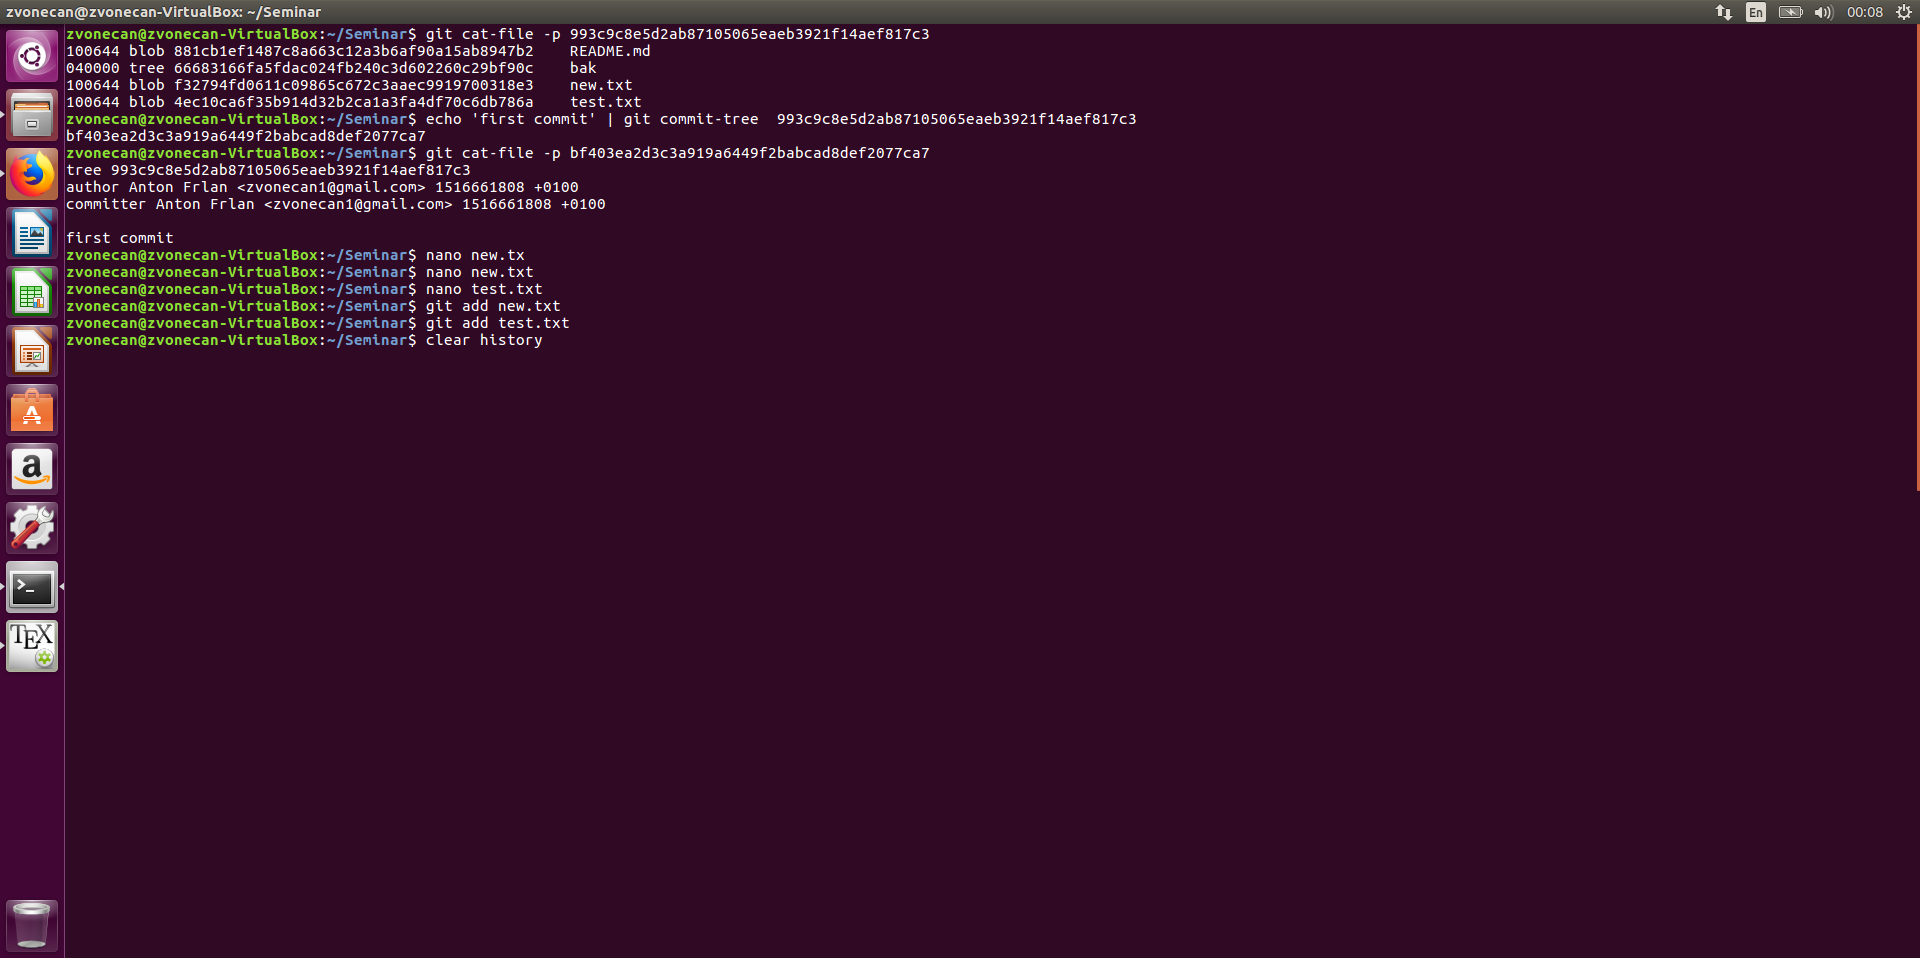
\includegraphics[width=1\textwidth]{./slike/sedma_slika.jpg}
	\end{figure}
\end{itemize}
\end{frame}
\begin{frame}{Branching}
	\begin{itemize}
	\item Jedna on najbitnijih stvari u gitu je grananje.
	\item Ono omogucuje razvijanje i debugiranje zasebnih featura bez remecenja glavnog programa. 
	\item Za ovo se mogu koristi reference koje zamijene neki SHA-1 proizvoljnim imenom i odonda se toj novoj grani moze pristupati tim imenom, to jest prati HEAD te grane.
	\end{itemize}
	
\end{frame}
\begin{frame}{Branching}
\begin{figure}
		\centering
	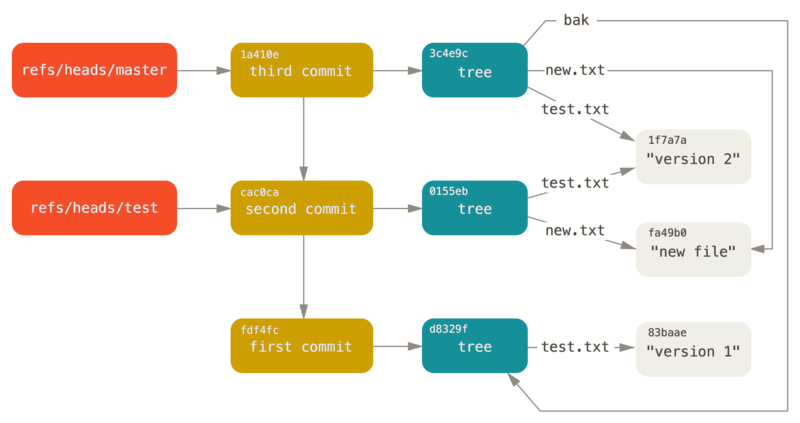
\includegraphics[width=1\textwidth]{./slike/a.jpg}
	\end{figure}
\end{frame}

\begin{frame}{Merge}
\begin{itemize}
	\item git merge usporeduje znakove na svim lokacijama i ako postoje mjesta na kojima nisu ista ih stavi odvoji i stavi jedno ispod drugog
\end{itemize}
\begin{figure}
		\centering
	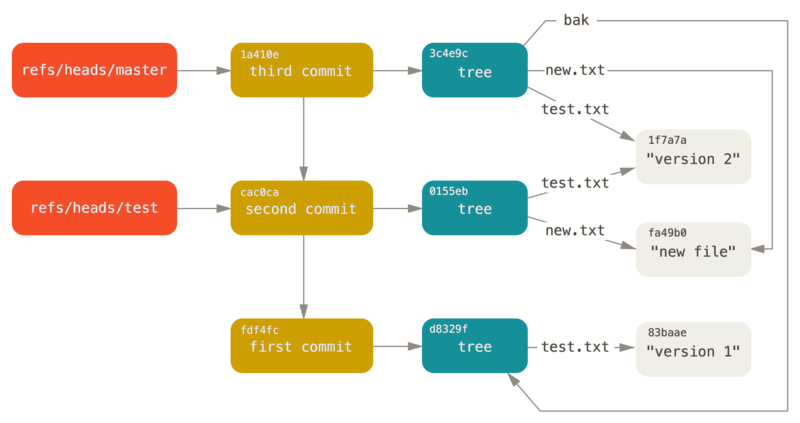
\includegraphics[width=1\textwidth]{./slike/a.jpg}
	\end{figure}
\end{frame}

\begin{frame}{HEAD}
	\begin{itemize}
	\item Odmah nakon prvog commita u gitu, prvi se i onda svaki sljedeci commit oznacuje kao HEAD.
	\item HEAD je referenca koja pokazuje na granu na kojoj se trenutno nalazimo, makar postojala samo jedna.
	\end{itemize}
\end{frame}
\begin{frame}{Tags}
	\begin{itemize}
	\item Tagovi su vrsta referenci i postoje lightweight and annoted.
	\begin{itemize}
	\item Lightweight su vrsta referenci koji se ne micu, umjesto ostajuci na jednom commitu
	\item Annoted su slozeniji tagovi koji stvore vlastiti objekt koji ima svoju referencu.
	\end{itemize}
	\end{itemize}
\end{frame}
\begin{frame}
	\begin{figure}
	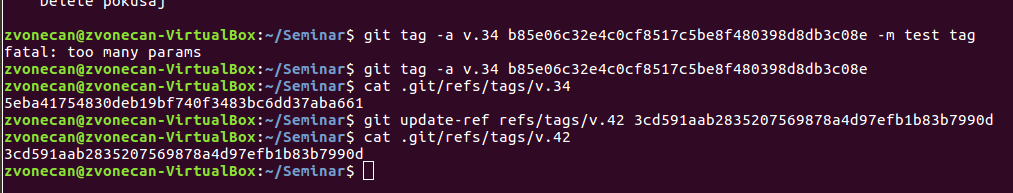
\includegraphics[width=1\textwidth]{./slike/tag.png}
	\end{figure}
\end{frame}
\begin{frame}{Remote}
	\begin{itemize}
	\item Remote je vrsta referenci koja se pokazuje na udaljeni repozitorij pomocu kojih se moze fetchati, pushati (poslati na repozitorij) i pullati (povuci s udaljenog repozitorija) sadrzaj tih repozitorija.  
	\end{itemize}
\end{frame}

\end{document}
>>>>>>> anton
